\begin{apendicesenv}

% Imprime uma página indicando o início dos apêndices
\partapendices

% Para cada apêndice, um \chapter


%#################################################################
\chapter{Grupo Focal} \label{ap:GRUPOFOCAL}
%#################################################################

%=================================================================
\section{Termo de Consentimento}
%=================================================================
    \begin{figure}
        \centering
        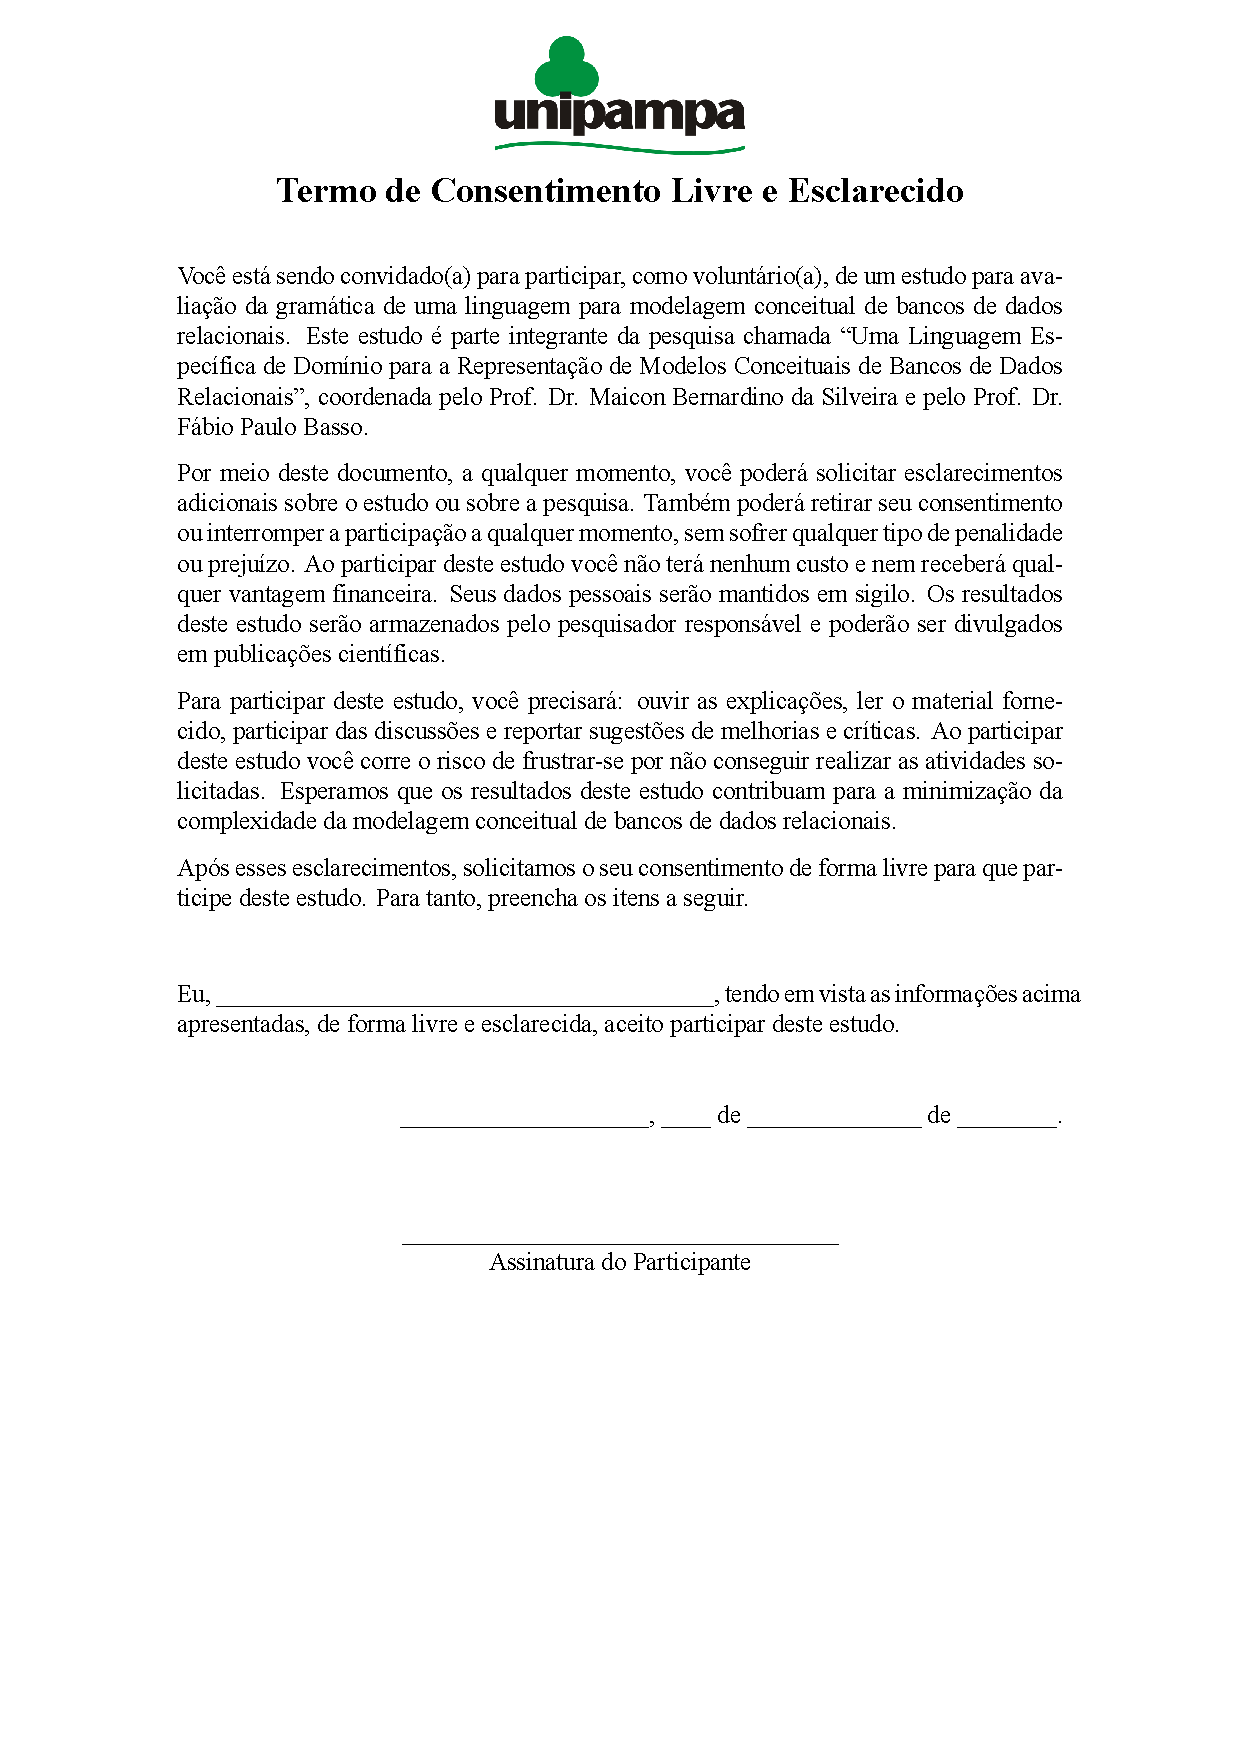
\includepdf[pages=-, frame=true, scale=0.65]{docsApend/grupoFocal/TermodeConsentimento} 
    \end{figure}
\newpage
%=================================================================
\section{Glossário de Termos}
%=================================================================
    \begin{figure}
        \centering
        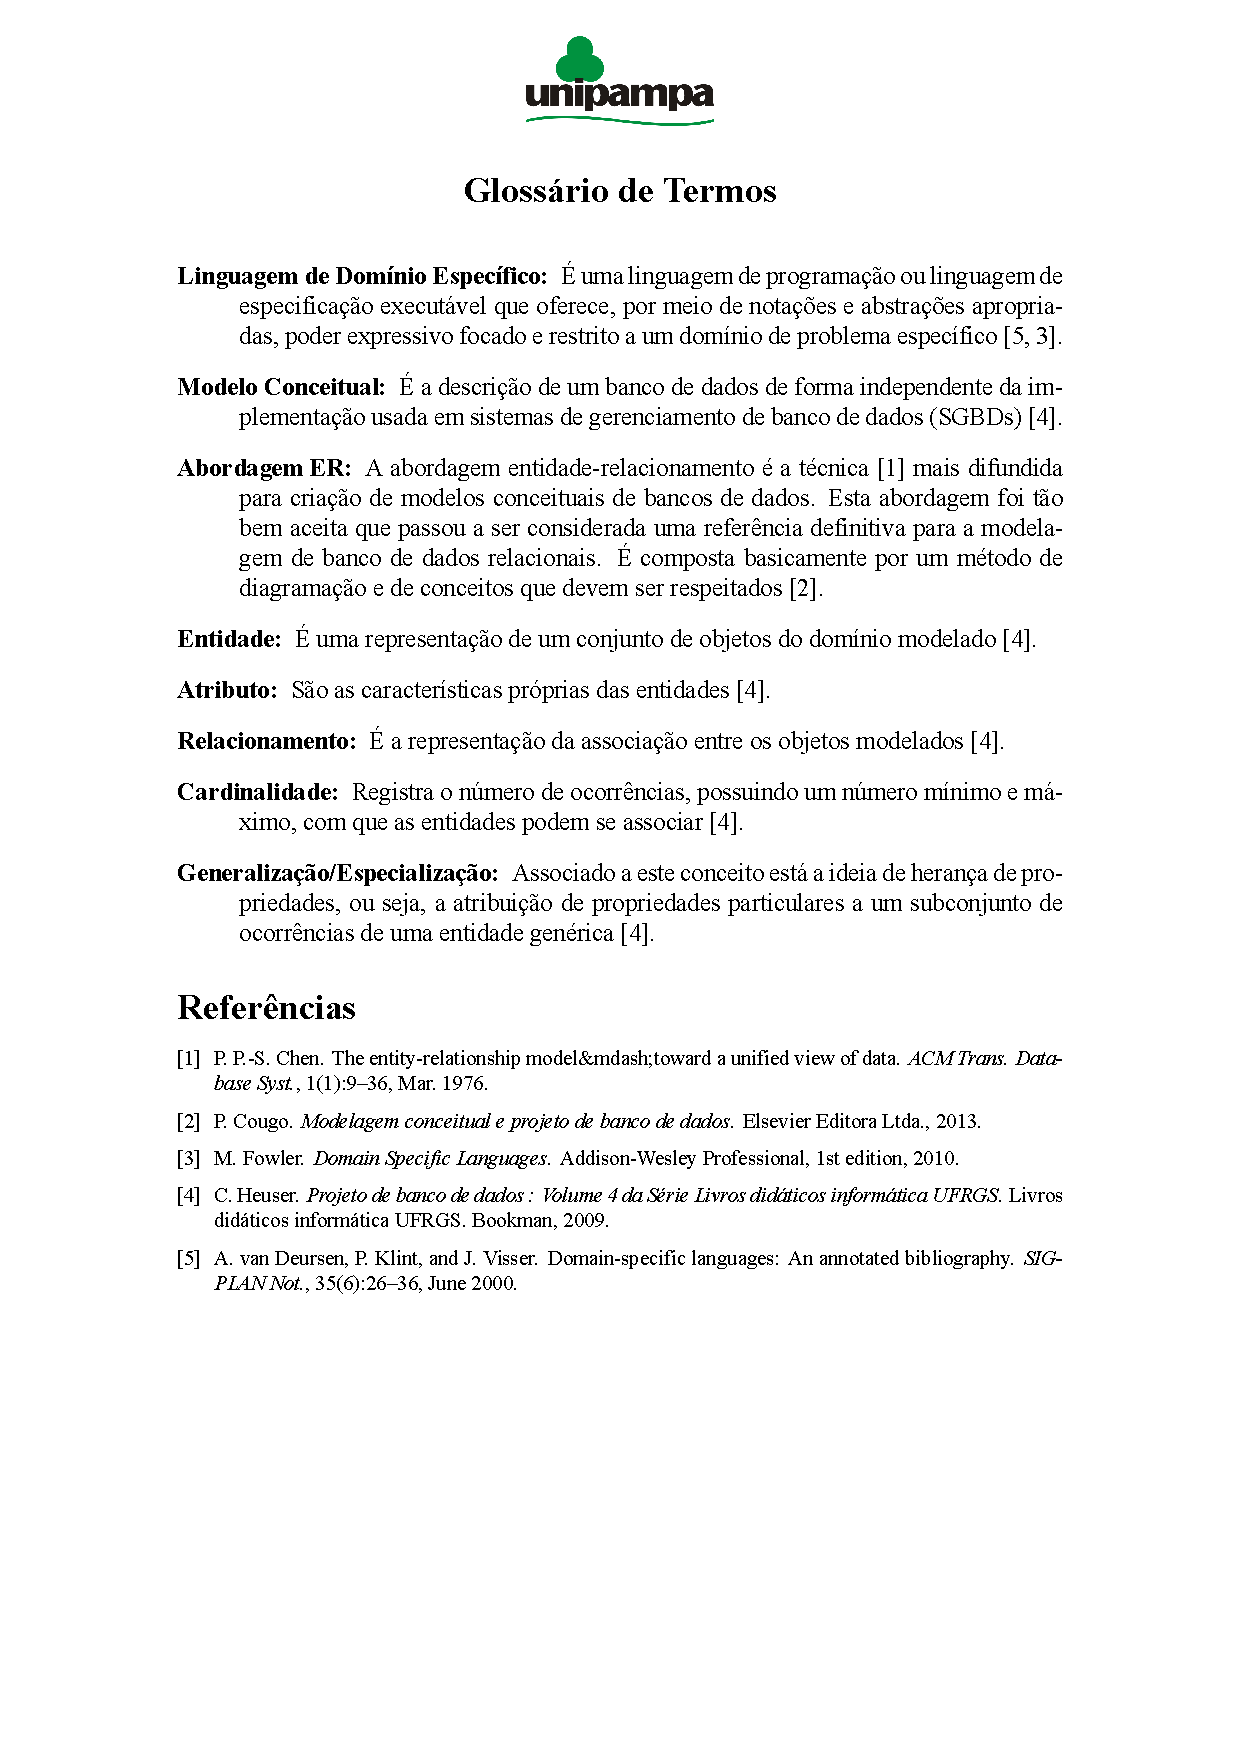
\includepdf[pages=-, frame=true, scale=0.65]{docsApend/grupoFocal/GlossariodeTermos} 
    \end{figure}
\newpage
%=================================================================
\section{Questionário de Perfil}
%=================================================================
    \begin{figure}
        \centering
        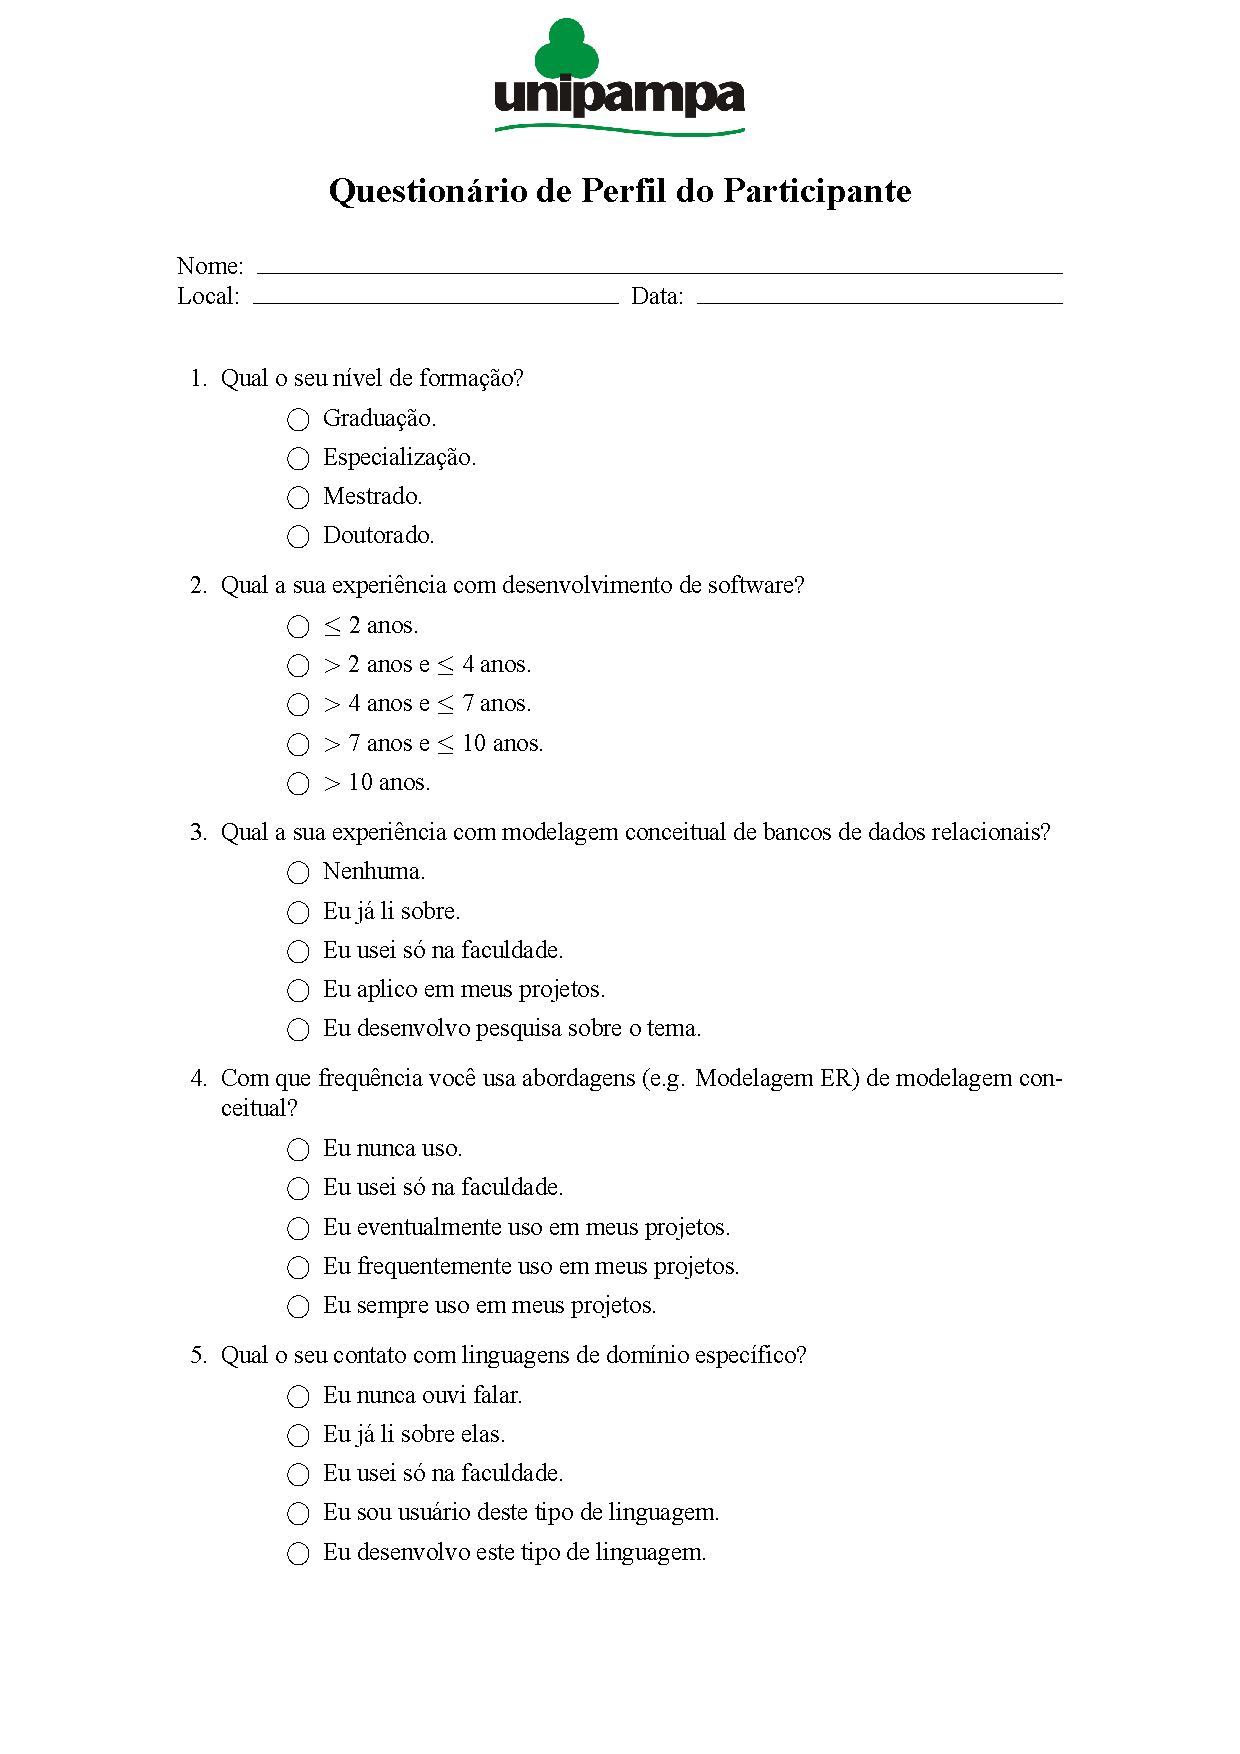
\includepdf[frame=true, pages=-, scale=0.65]{docsApend/grupoFocal/Perfil} 
    \end{figure}
\newpage
%=================================================================
\section{Roteiro}
%=================================================================
    \begin{figure}
        \centering
        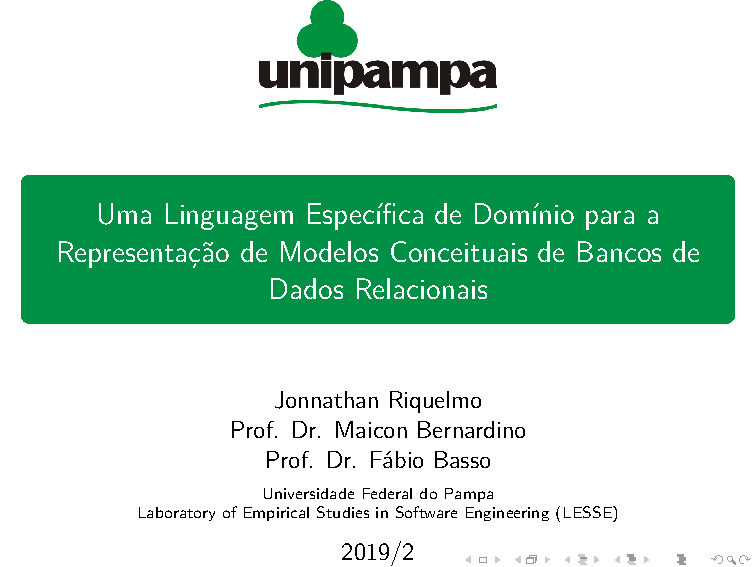
\includepdf[nup=4x5, pages=-, frame=true, scale=0.90]{docsApend/grupoFocal/Roteiro} 
    \end{figure}
\newpage
%=================================================================
\section{Discussão 1}
%=================================================================
    \begin{figure}[!htb]
        \centering
        \includepdf[pages=-, frame=true, scale=0.65]{docsApend/grupoFocal/Discussao1}
        % \includegraphics[scale=0.70]{docsApend/Discussao1.pdf}
    \end{figure}
\newpage
%=================================================================
\section{Discussão 2}
%=================================================================
    \begin{figure}
        \centering
        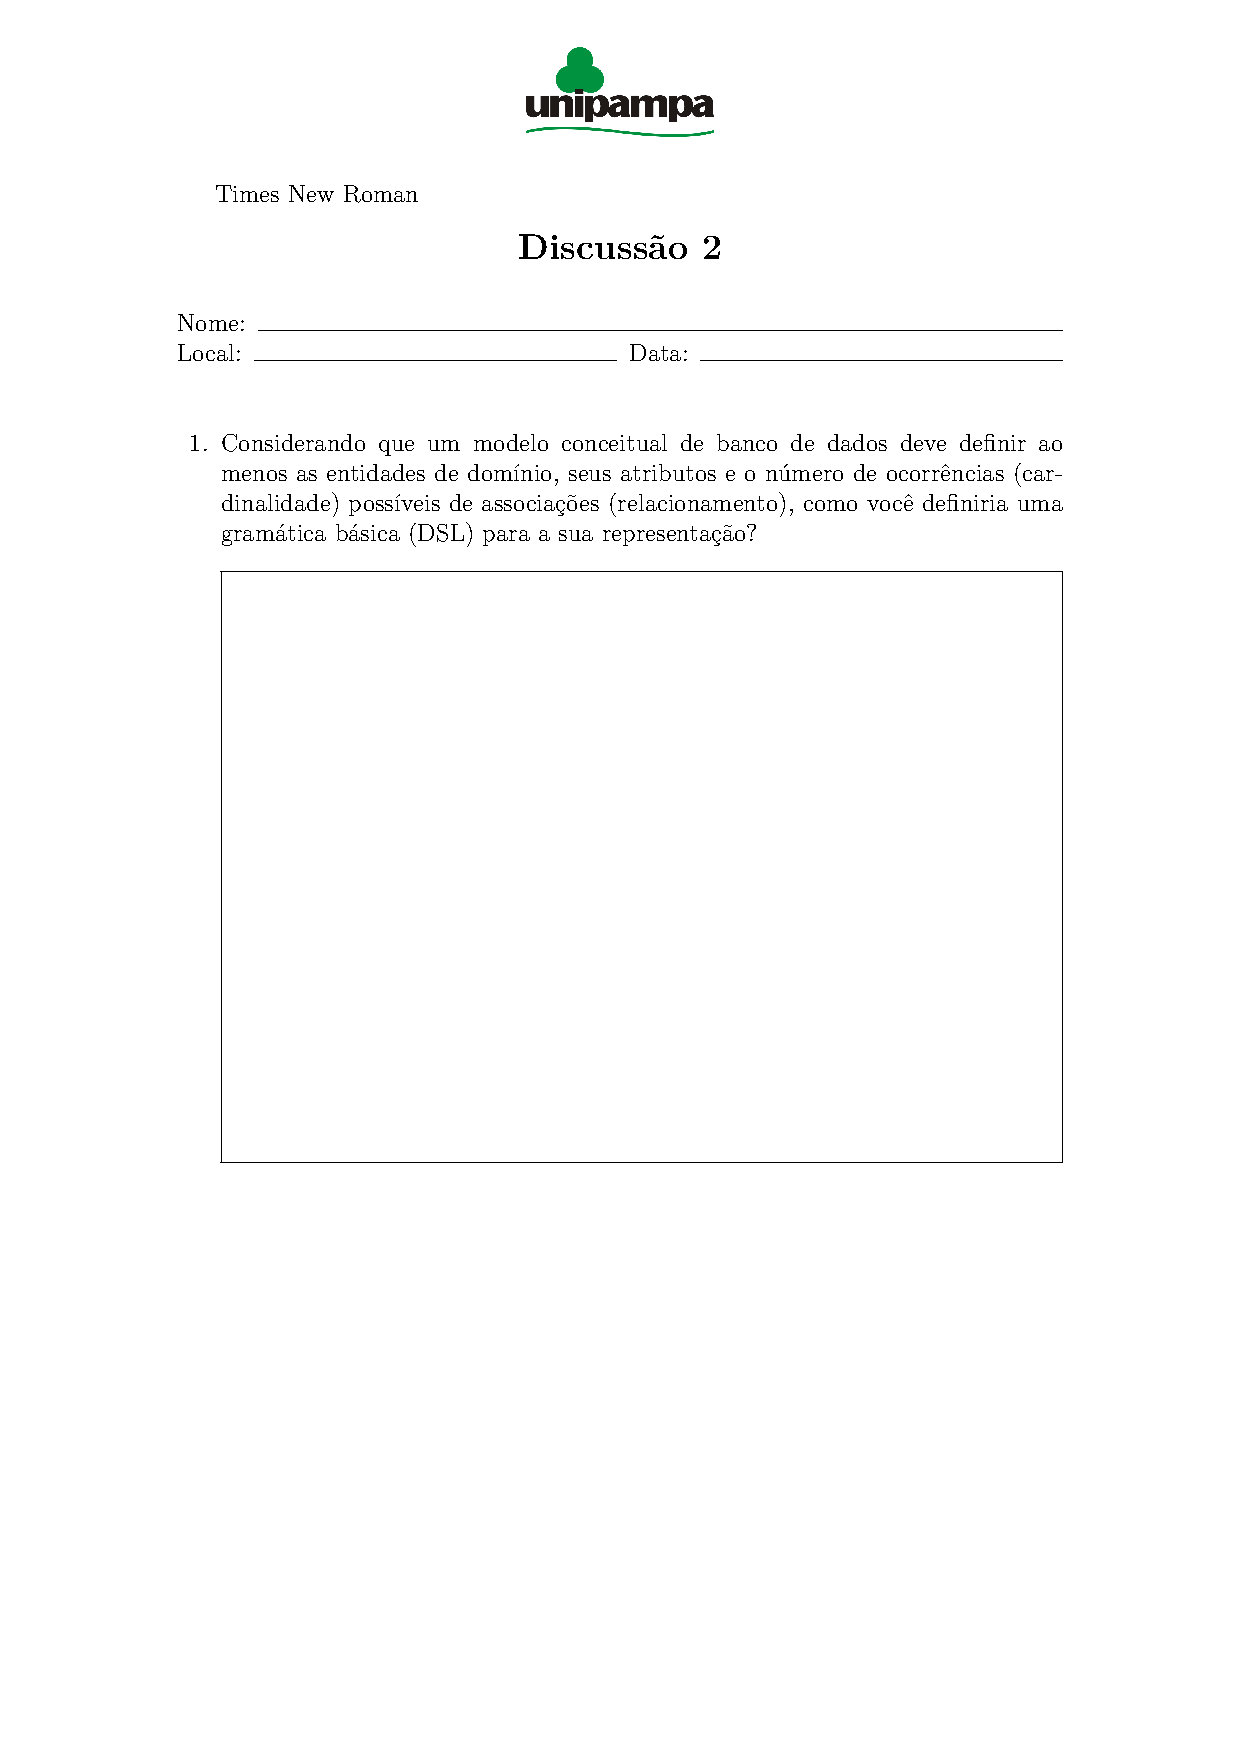
\includepdf[pages=-, frame=true, scale=0.65]{docsApend/grupoFocal/Discussao2} 
    \end{figure}
\newpage
%=================================================================
\section{Discussão 3}
%=================================================================
    \begin{figure}
        \centering
        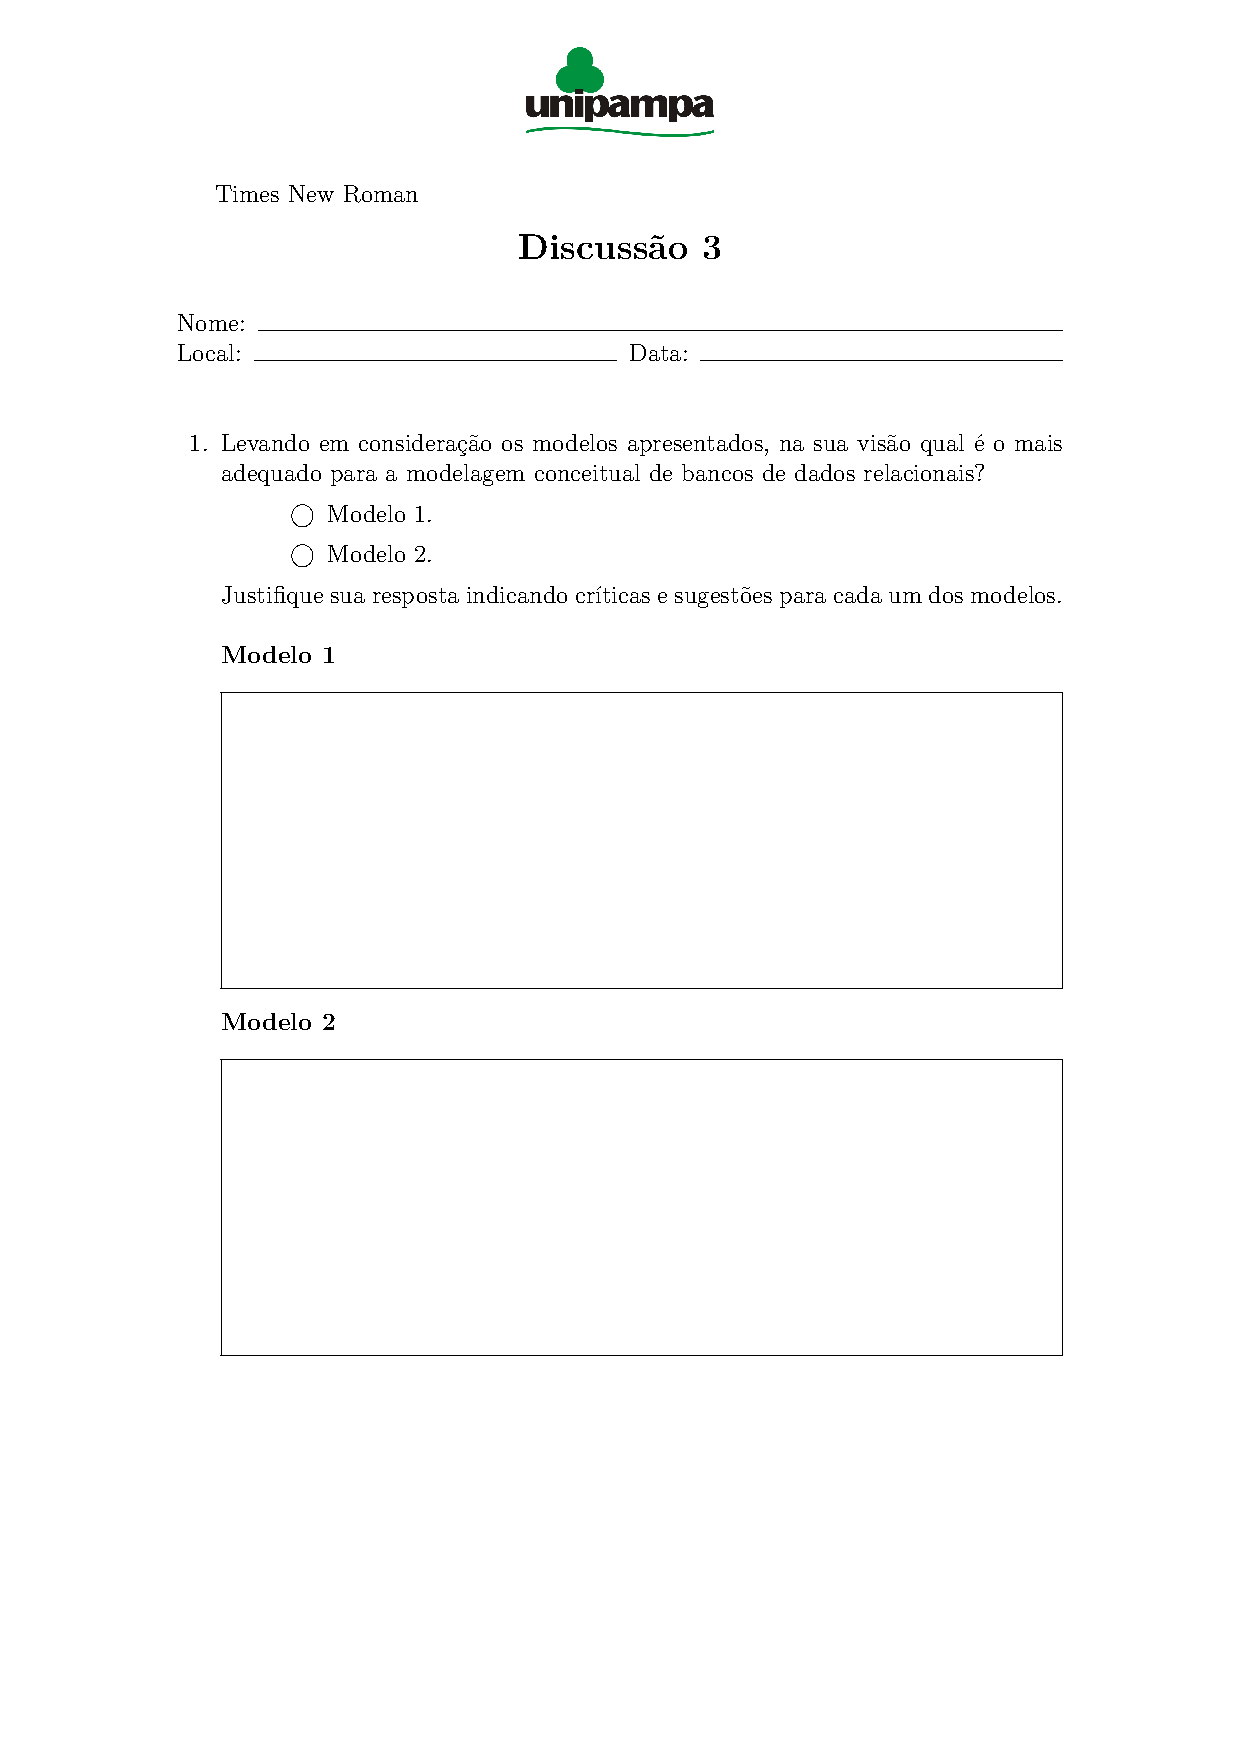
\includepdf[pages=-, frame=true, scale=0.65]{docsApend/grupoFocal/Discussao3} 
    \end{figure}
\newpage
%=================================================================
\section{Modelos da DSL}
%=================================================================
    \begin{figure}
        \centering
        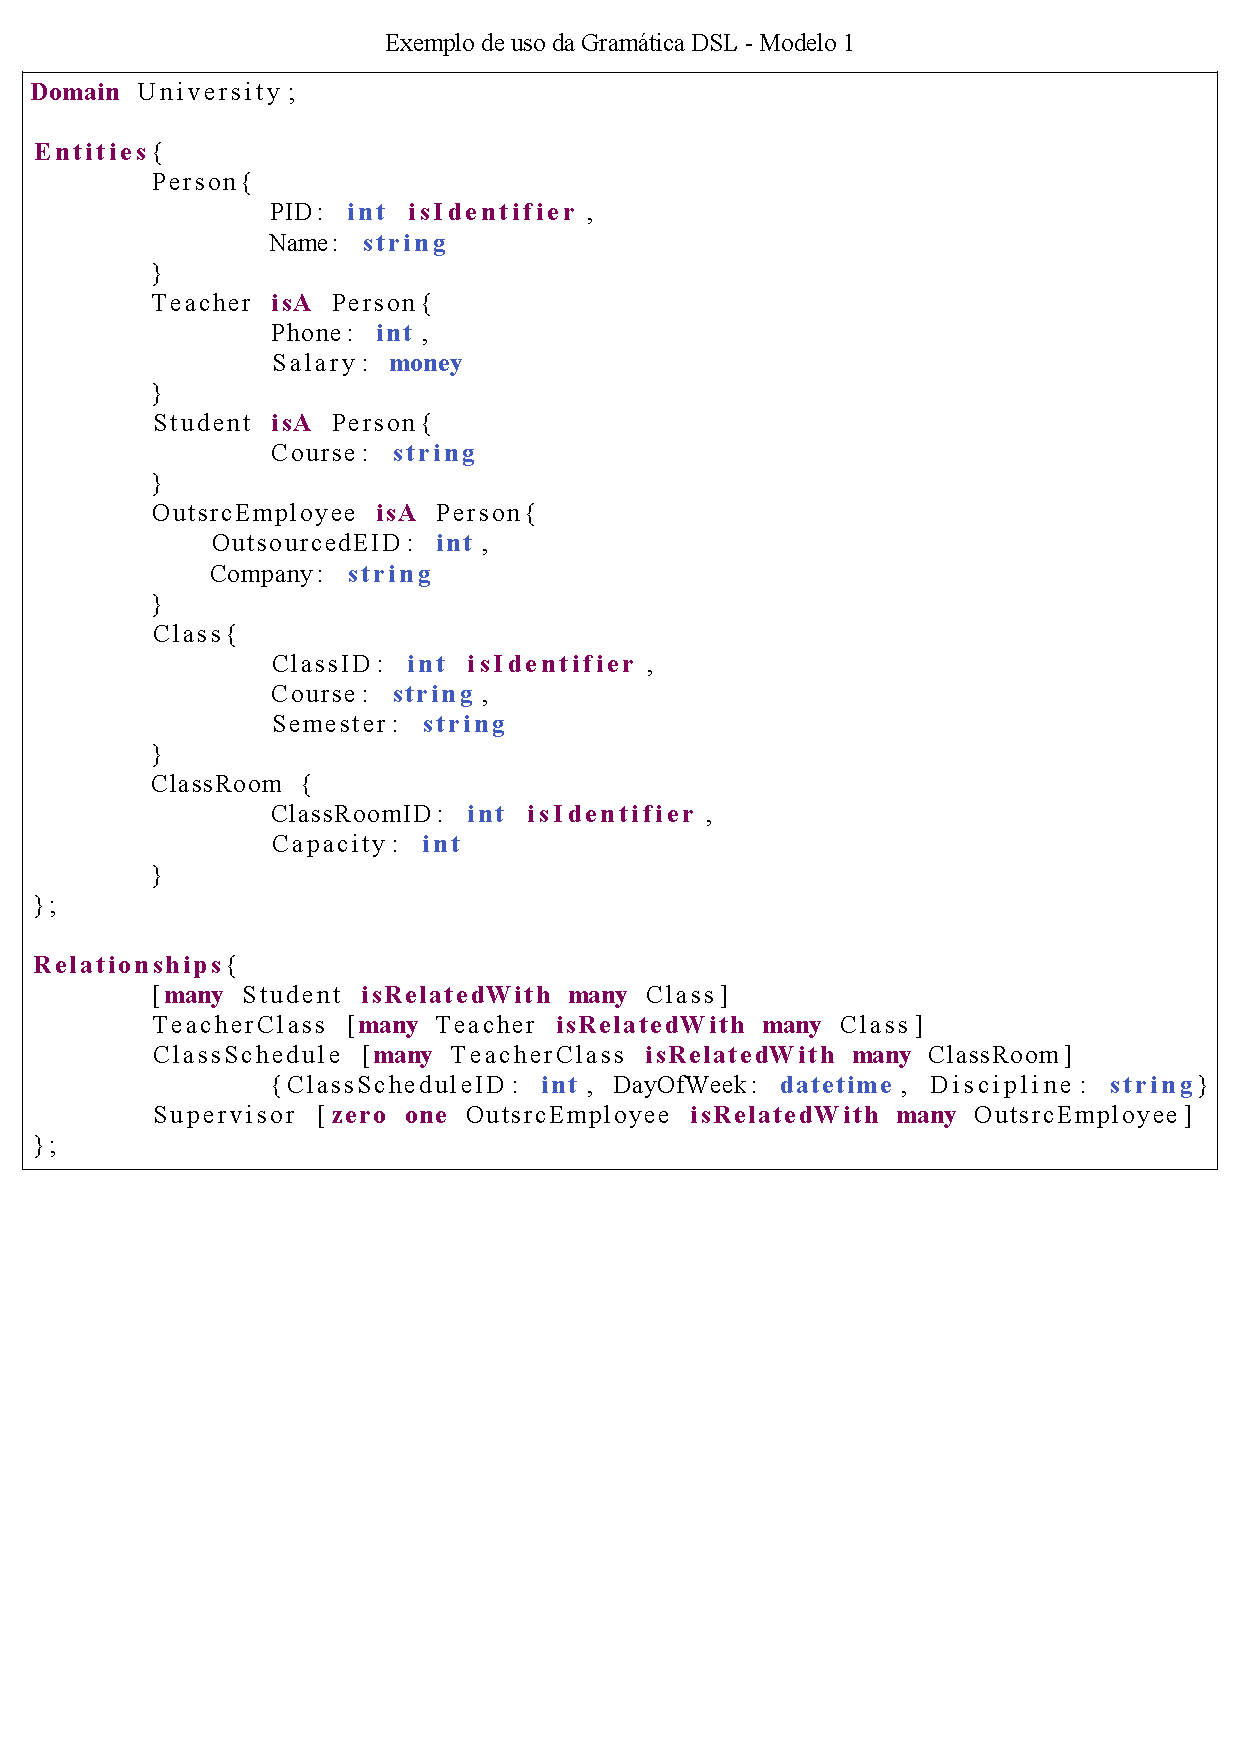
\includepdf[nup=2x1, pages=-, scale=0.90]{docsApend/grupoFocal/ModelosDSL} 
    \end{figure}
\newpage

%#################################################################
\chapter{Experimento Controlado} \label{EXPERIMENTOCONTROL}
%#################################################################

%=================================================================
\section{Termo de Consentimento}
%=================================================================
    \begin{figure}
        \centering
        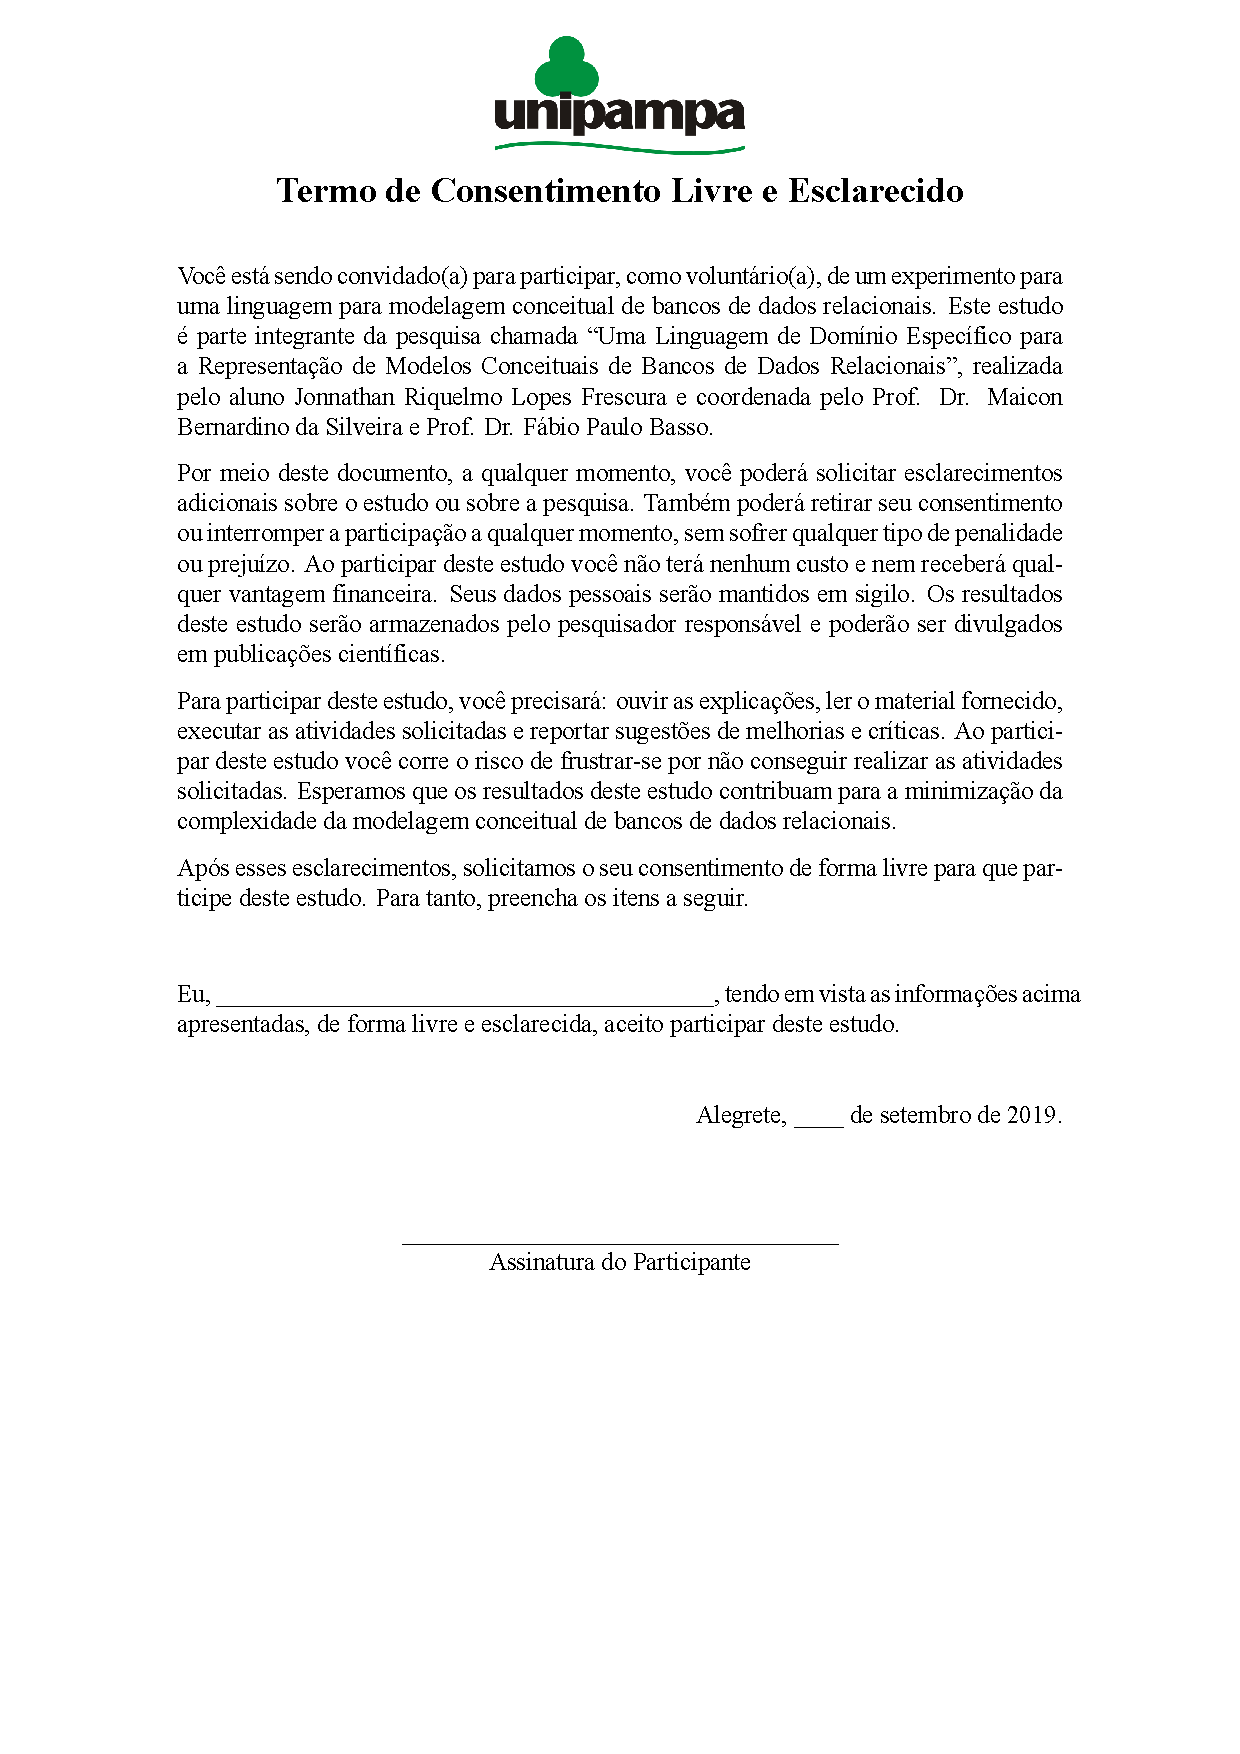
\includepdf[pages=-, frame=true, scale=0.65]{docsApend/expControl/Termo} 
    \end{figure}
\newpage
%=================================================================
\section{Glossário de Termos}
%=================================================================
    \begin{figure}
        \centering
        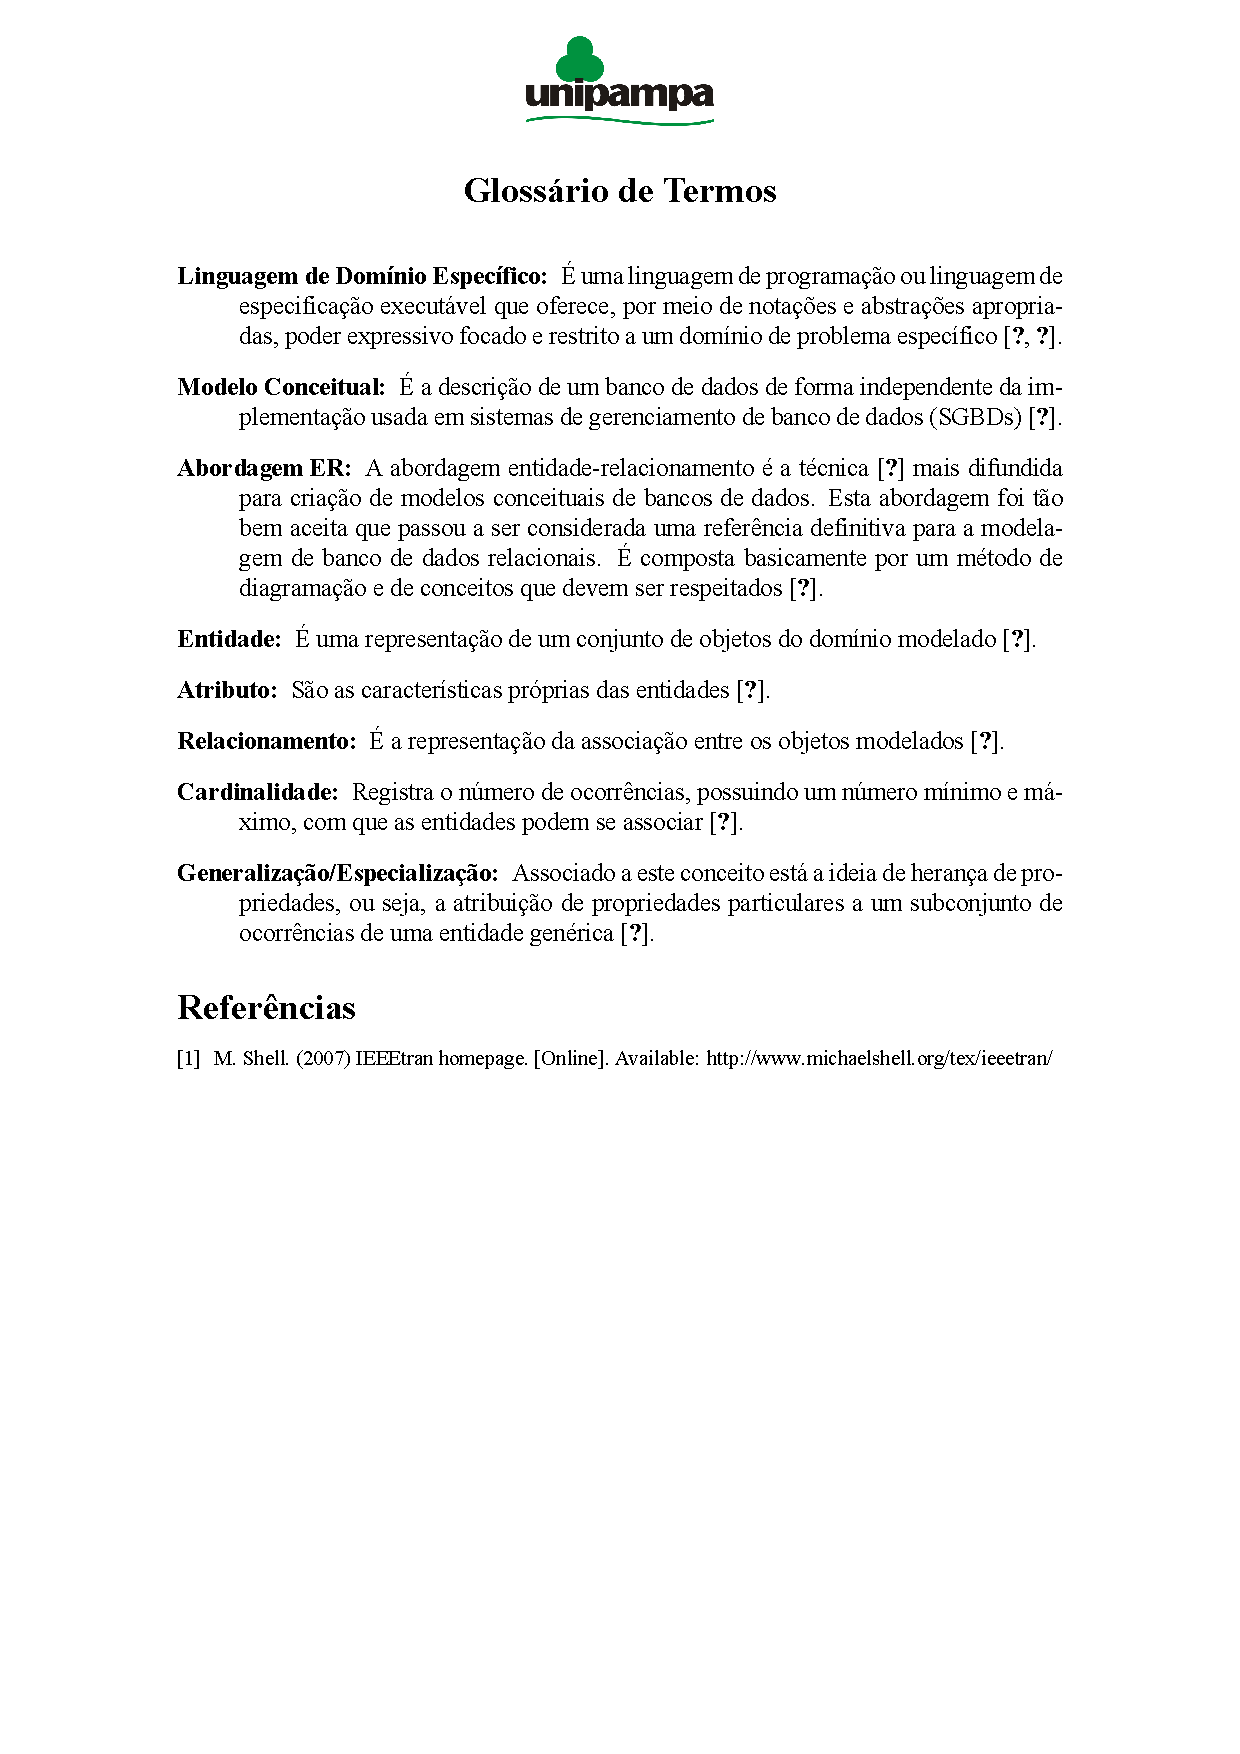
\includepdf[pages=-, frame=true, scale=0.65]{docsApend/expControl/Glossario} 
    \end{figure}
\newpage
%=================================================================
\section{Questionário de Perfil}
%=================================================================
    \begin{figure}
        \centering
        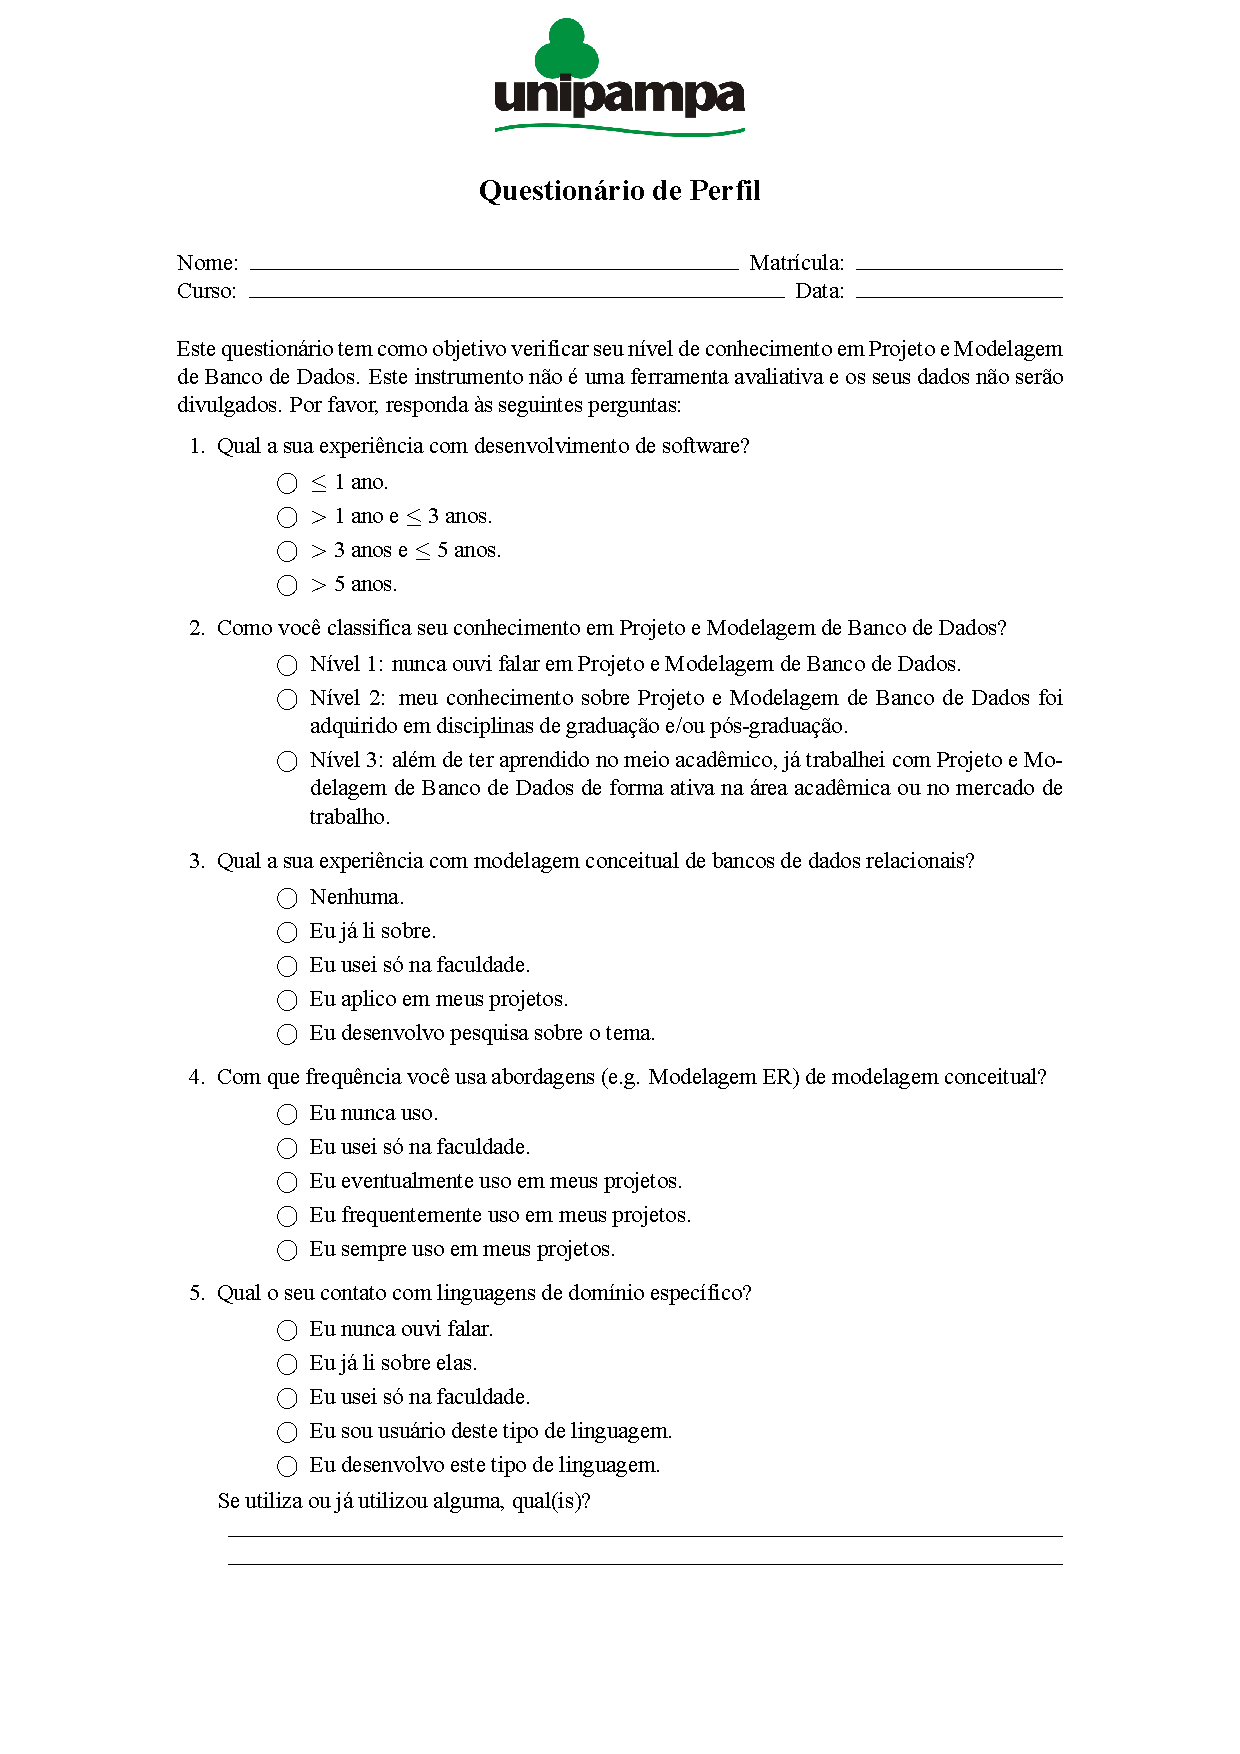
\includepdf[pages=-, frame=true, scale=0.65]{docsApend/expControl/Perfil} 
    \end{figure}
\newpage
%=================================================================
\section{Instruções BRModelo}
%=================================================================
    \begin{figure}
        \centering
        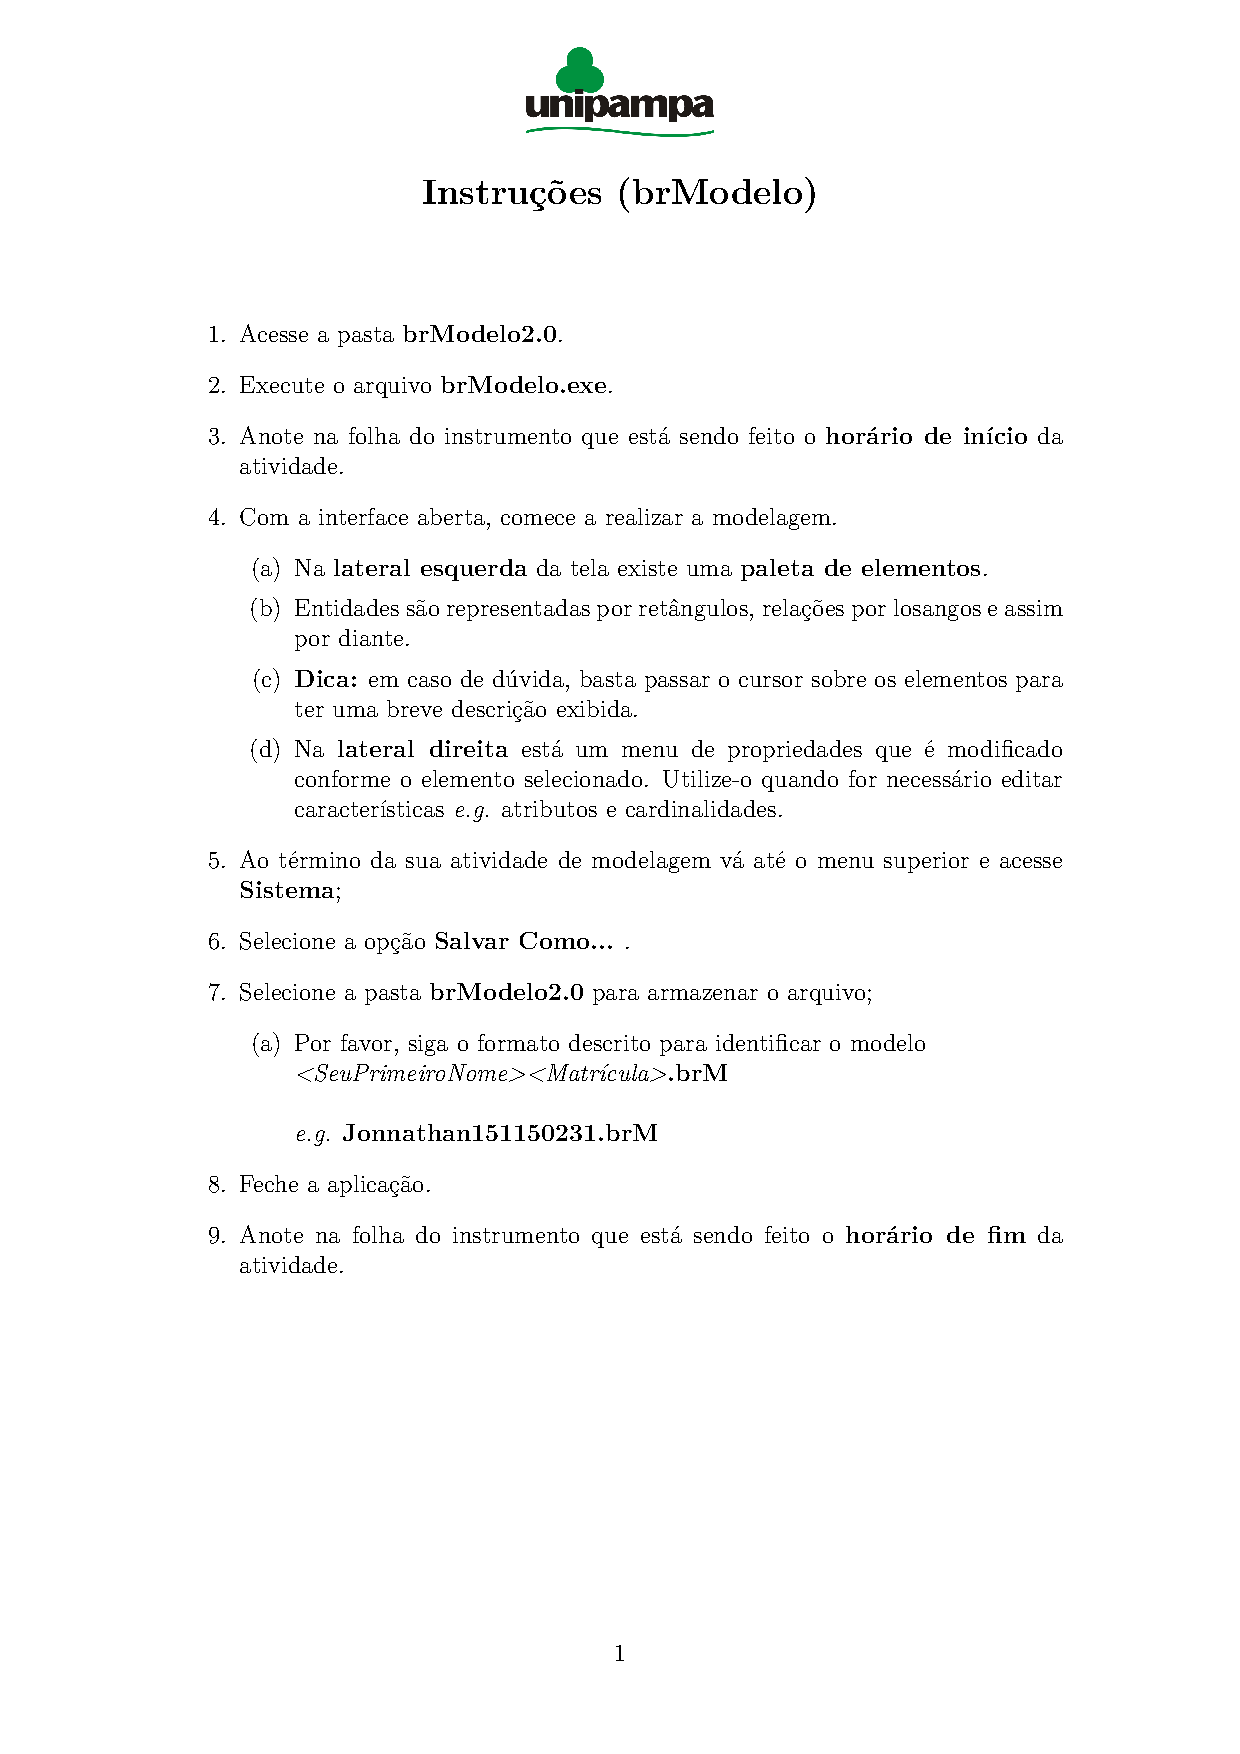
\includepdf[nup=2x1, pages=-, frame=true, scale=0.90]{docsApend/expControl/PassoBrModelo} 
    \end{figure}
\newpage
%=================================================================
\section{Instruções ERDSL}
%=================================================================
    \begin{figure}
        \centering
        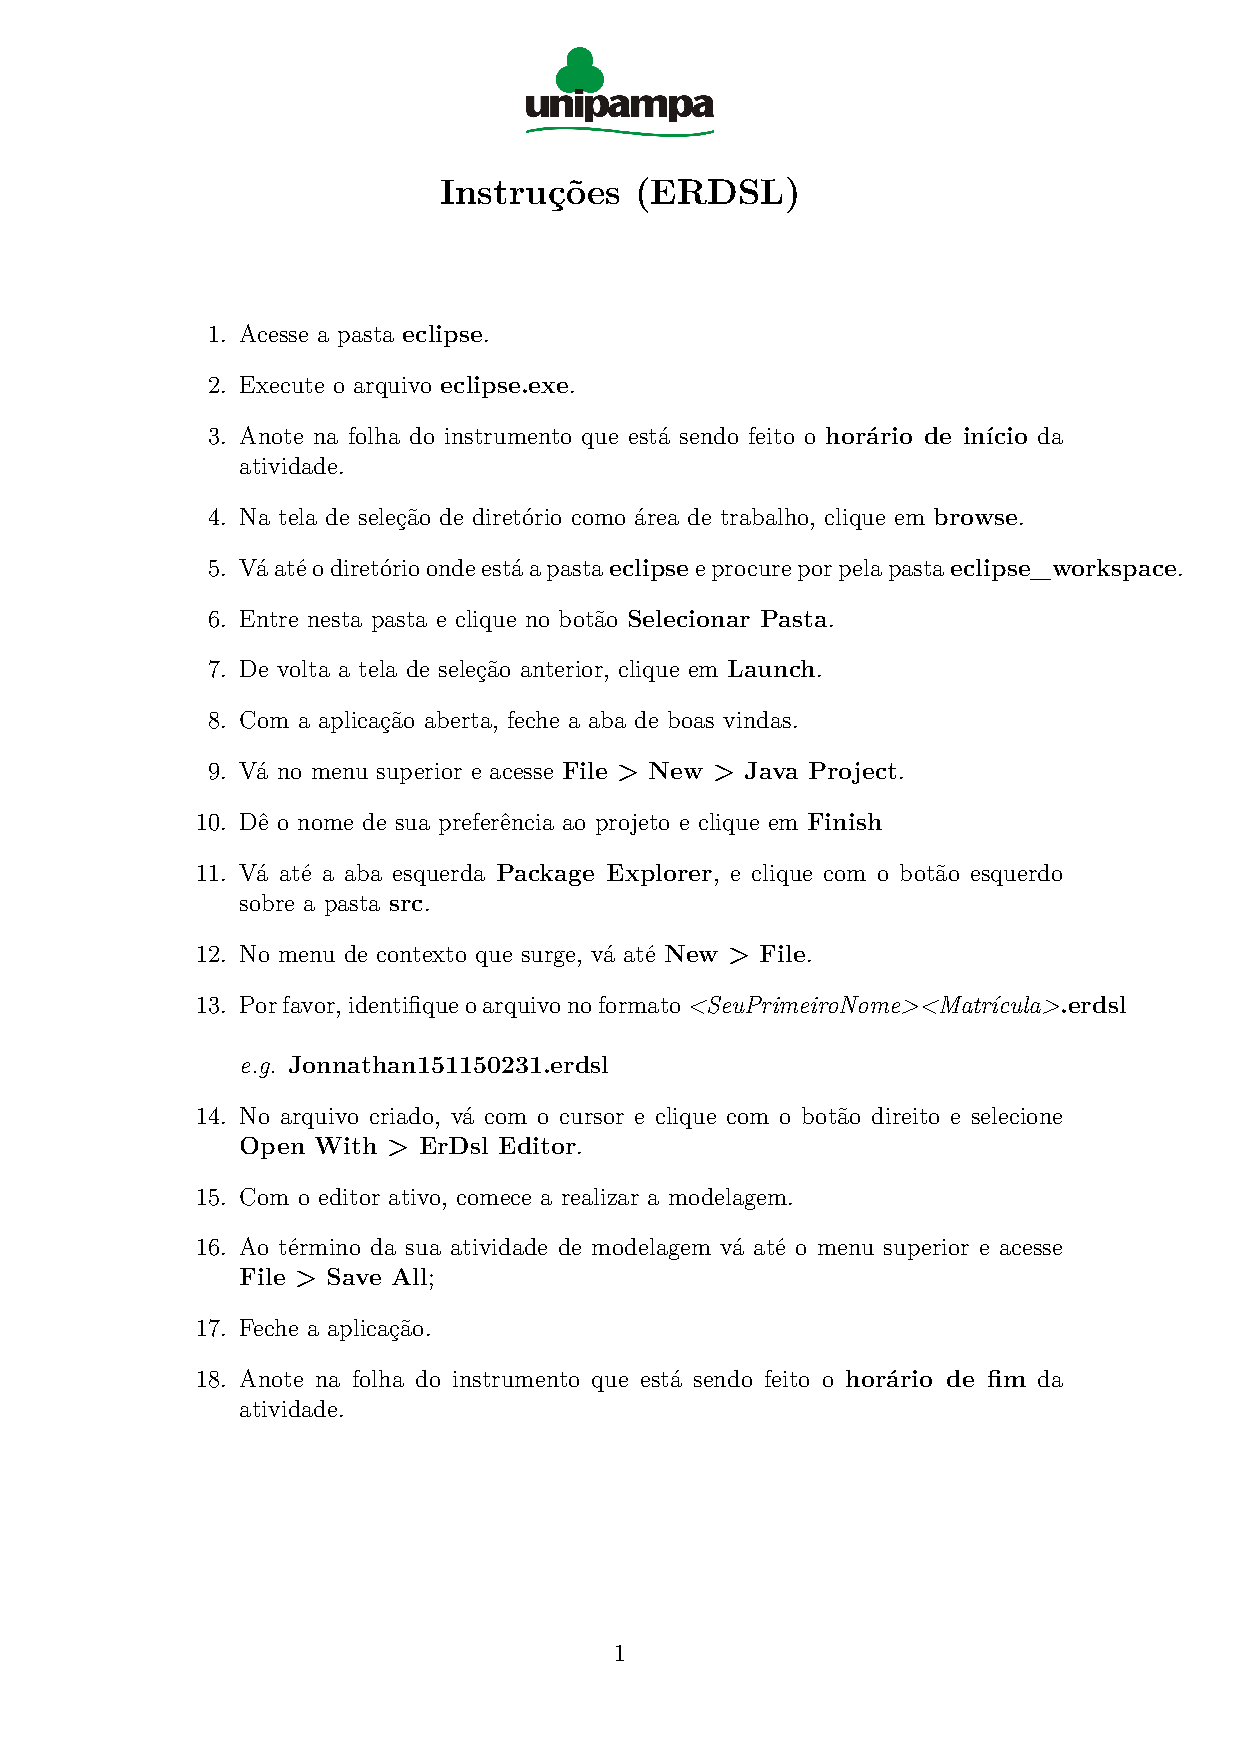
\includepdf[nup=2x1, pages=-, frame=true, scale=0.90]{docsApend/expControl/PassoERDSL} 
    \end{figure}
\newpage
%=================================================================
\section{Instrumento 1}
%=================================================================
    \begin{figure}
        \centering
        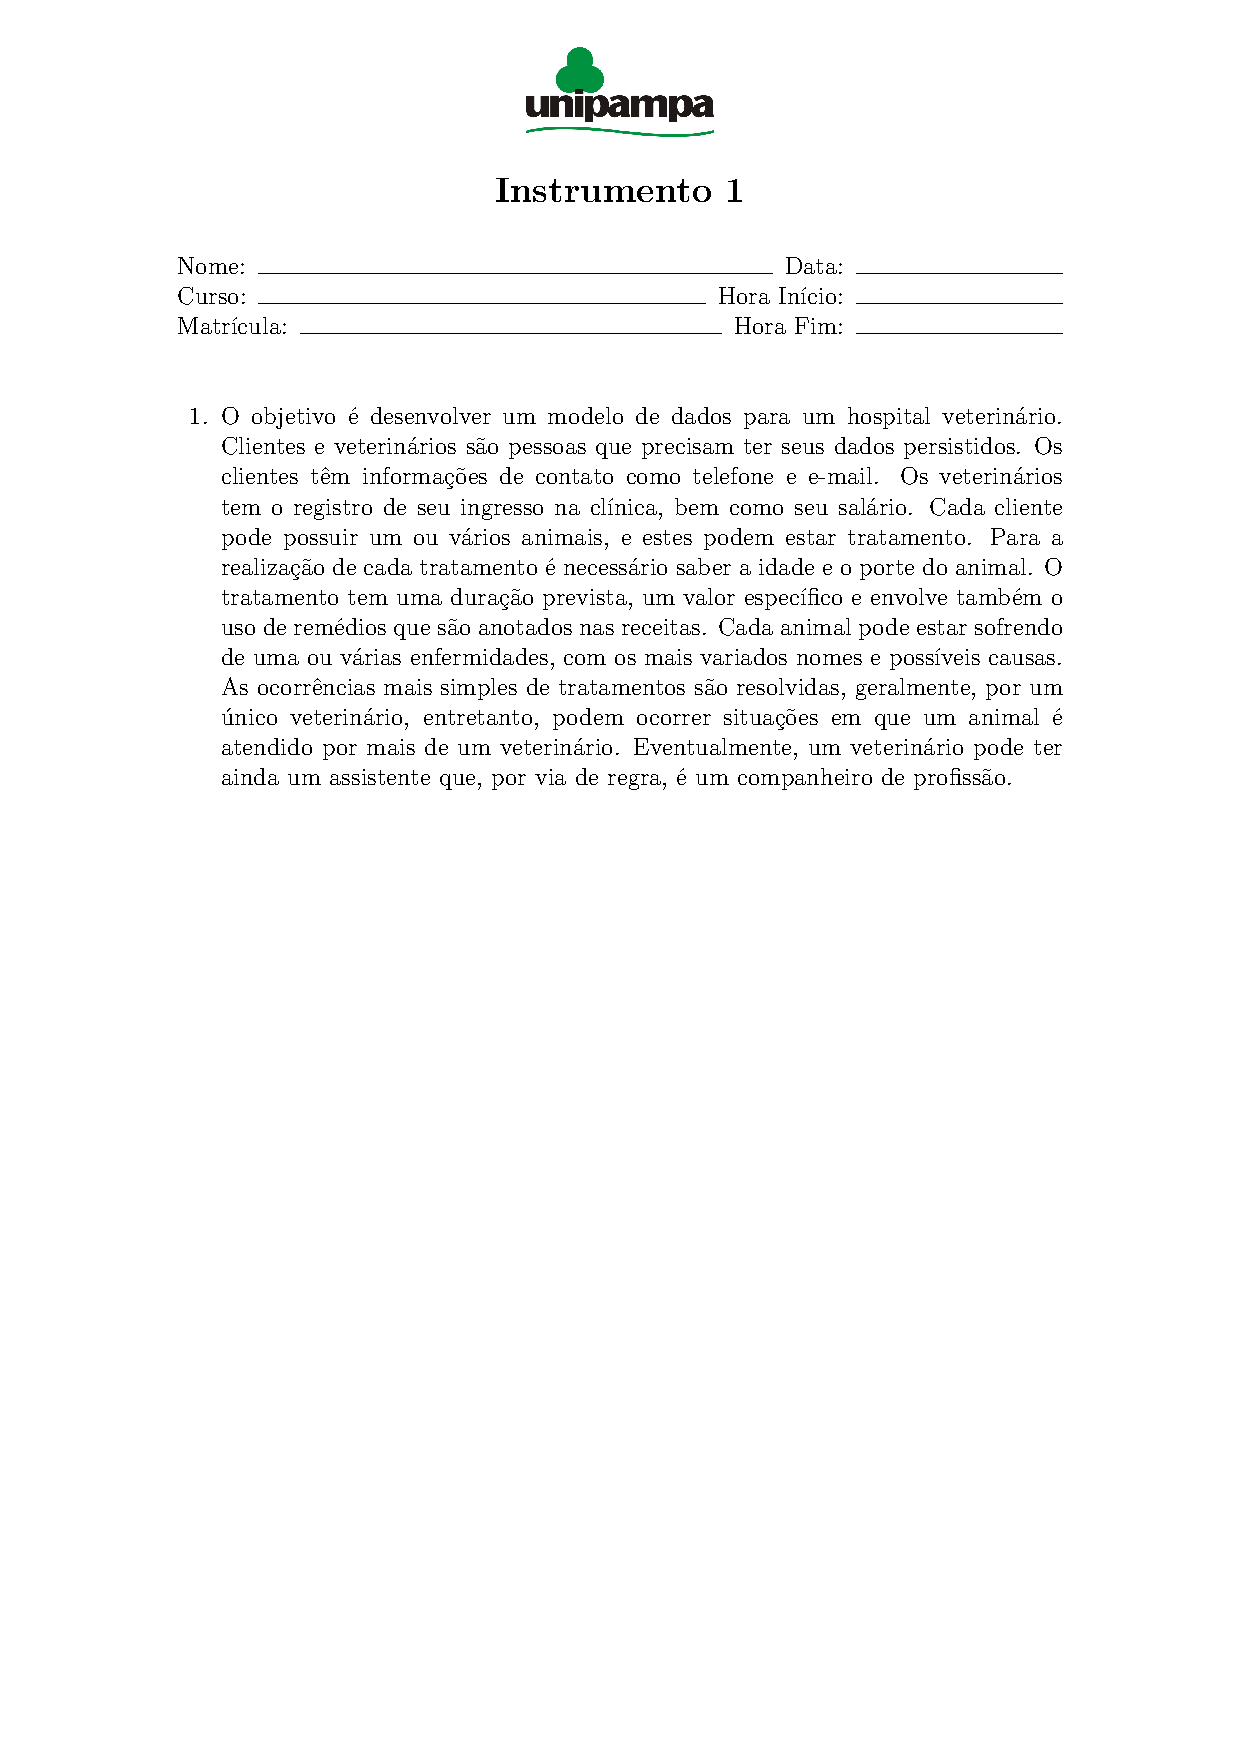
\includepdf[pages=-, frame=true, scale=0.65]{docsApend/expControl/Instrumento1} 
    \end{figure}
\newpage
%=================================================================
\section{Instrumento 2}
%=================================================================
    \begin{figure}
        \centering
        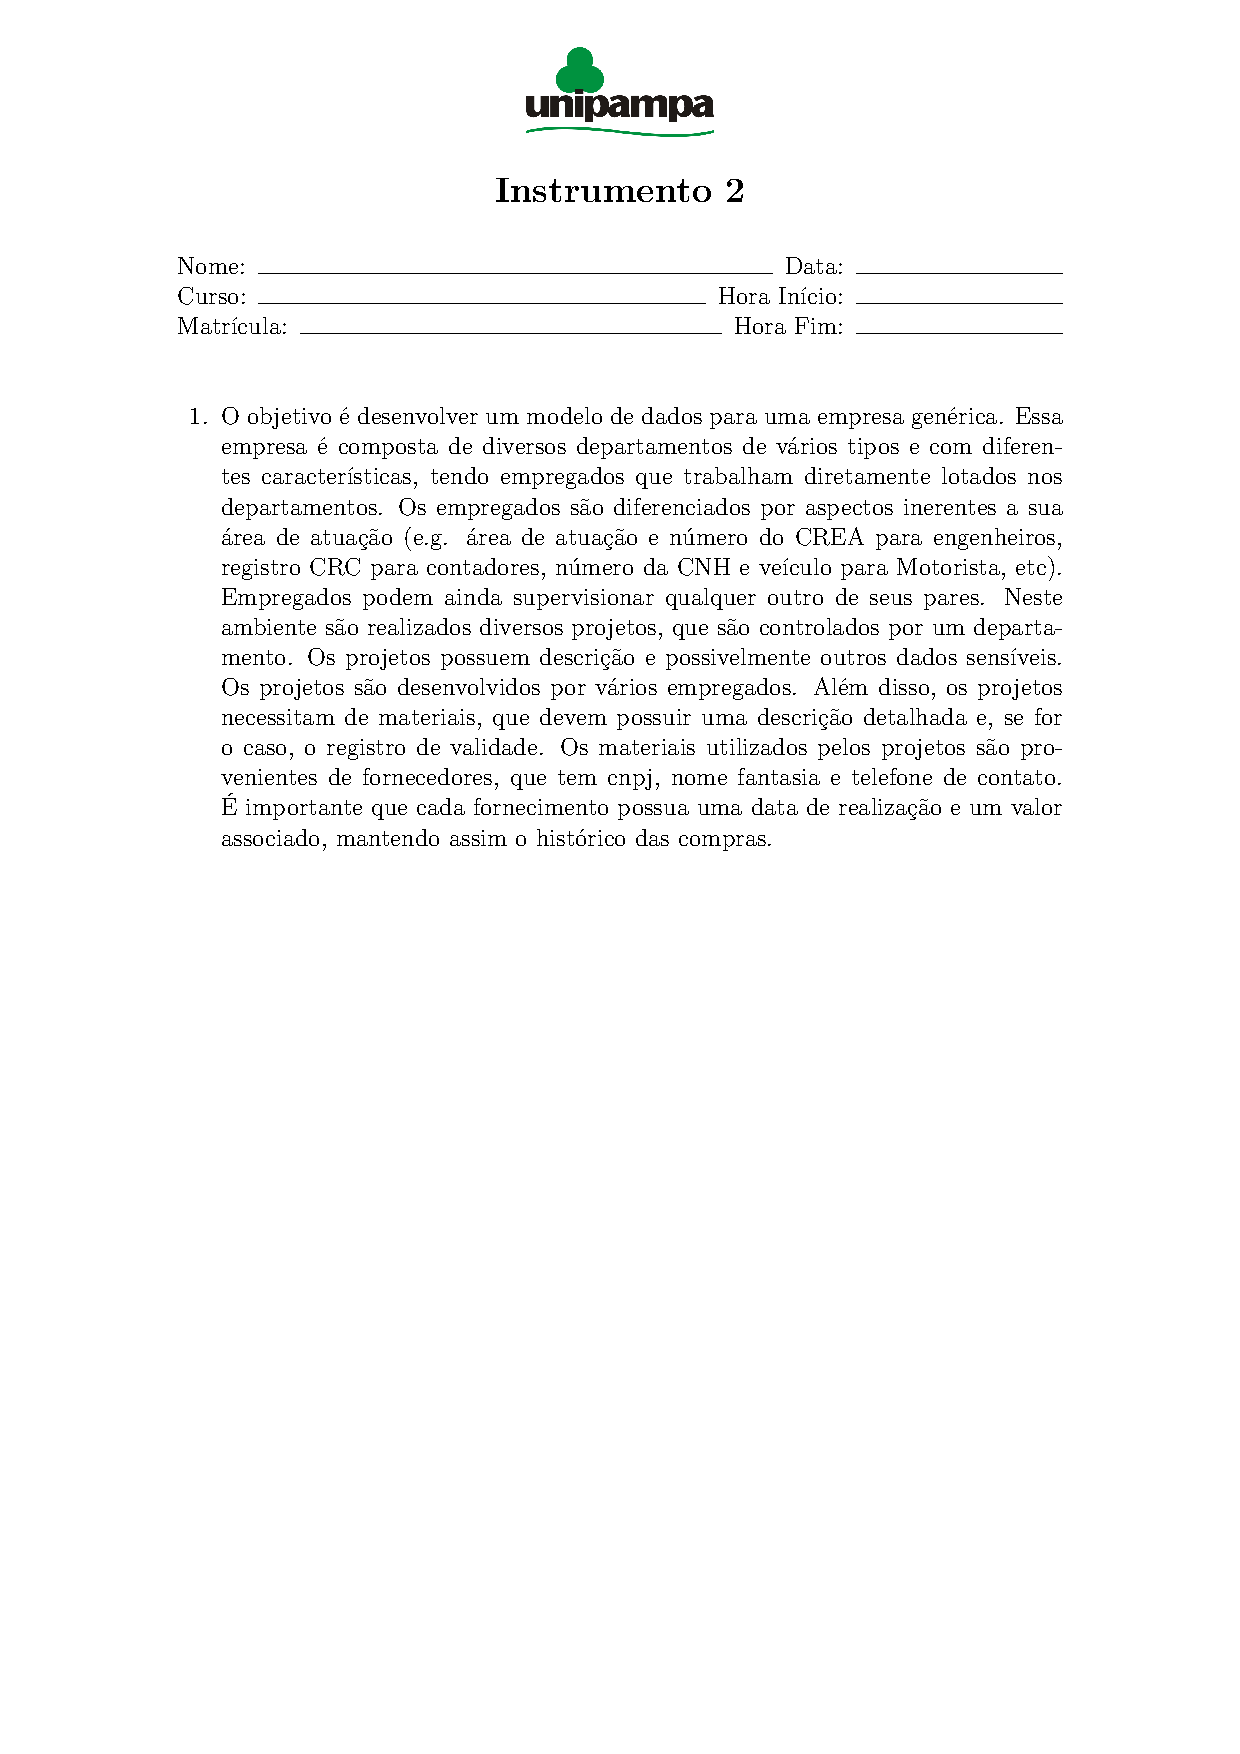
\includepdf[pages=-, frame=true, scale=0.65]{docsApend/expControl/Instrumento2} 
    \end{figure}
\newpage
%=================================================================
\section{Instrumento 3}
%=================================================================
    \begin{figure}
        \centering
        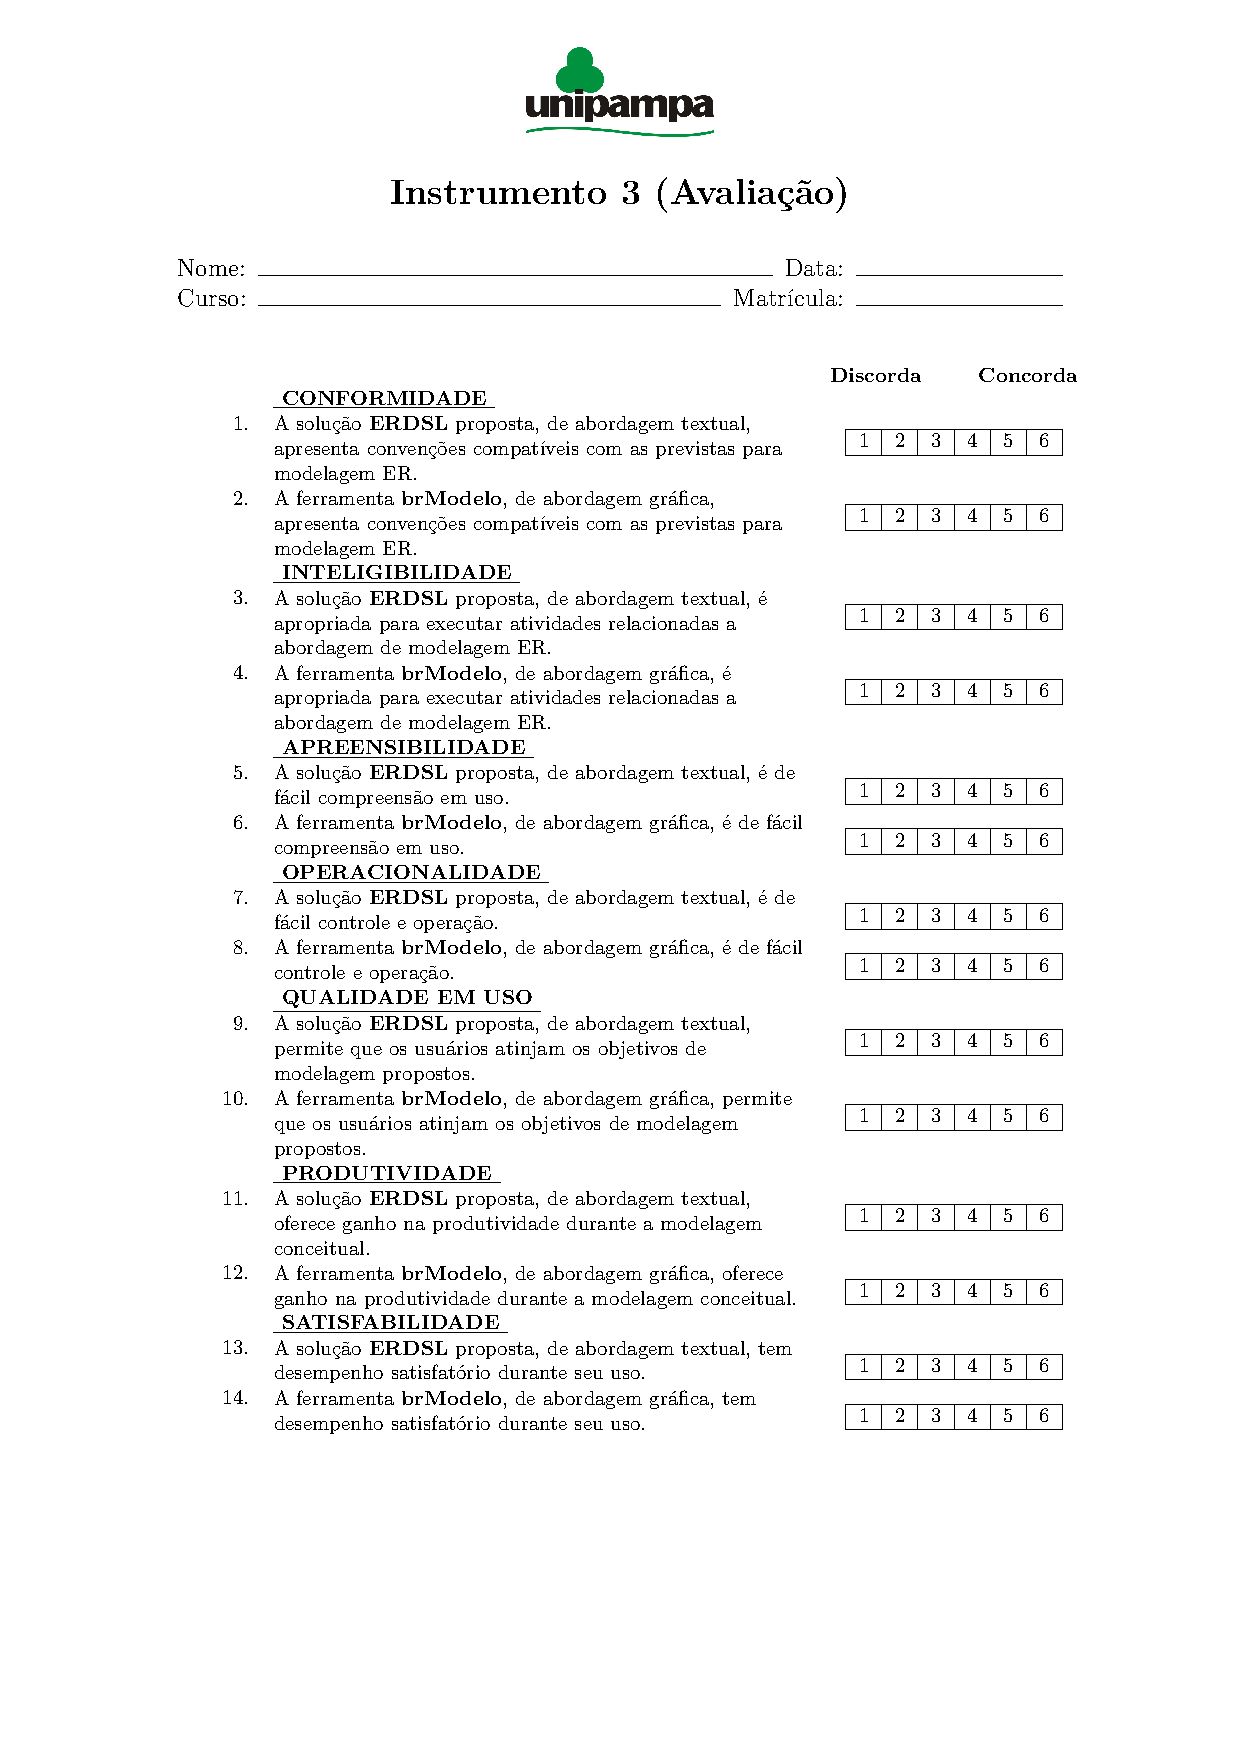
\includepdf[nup=2x1, pages=-, frame=true, scale=0.90]{docsApend/expControl/Instrumento3} 
    \end{figure}
\newpage
%=================================================================
\section{Instrumento 4}
%=================================================================
    \begin{figure}
        \centering
        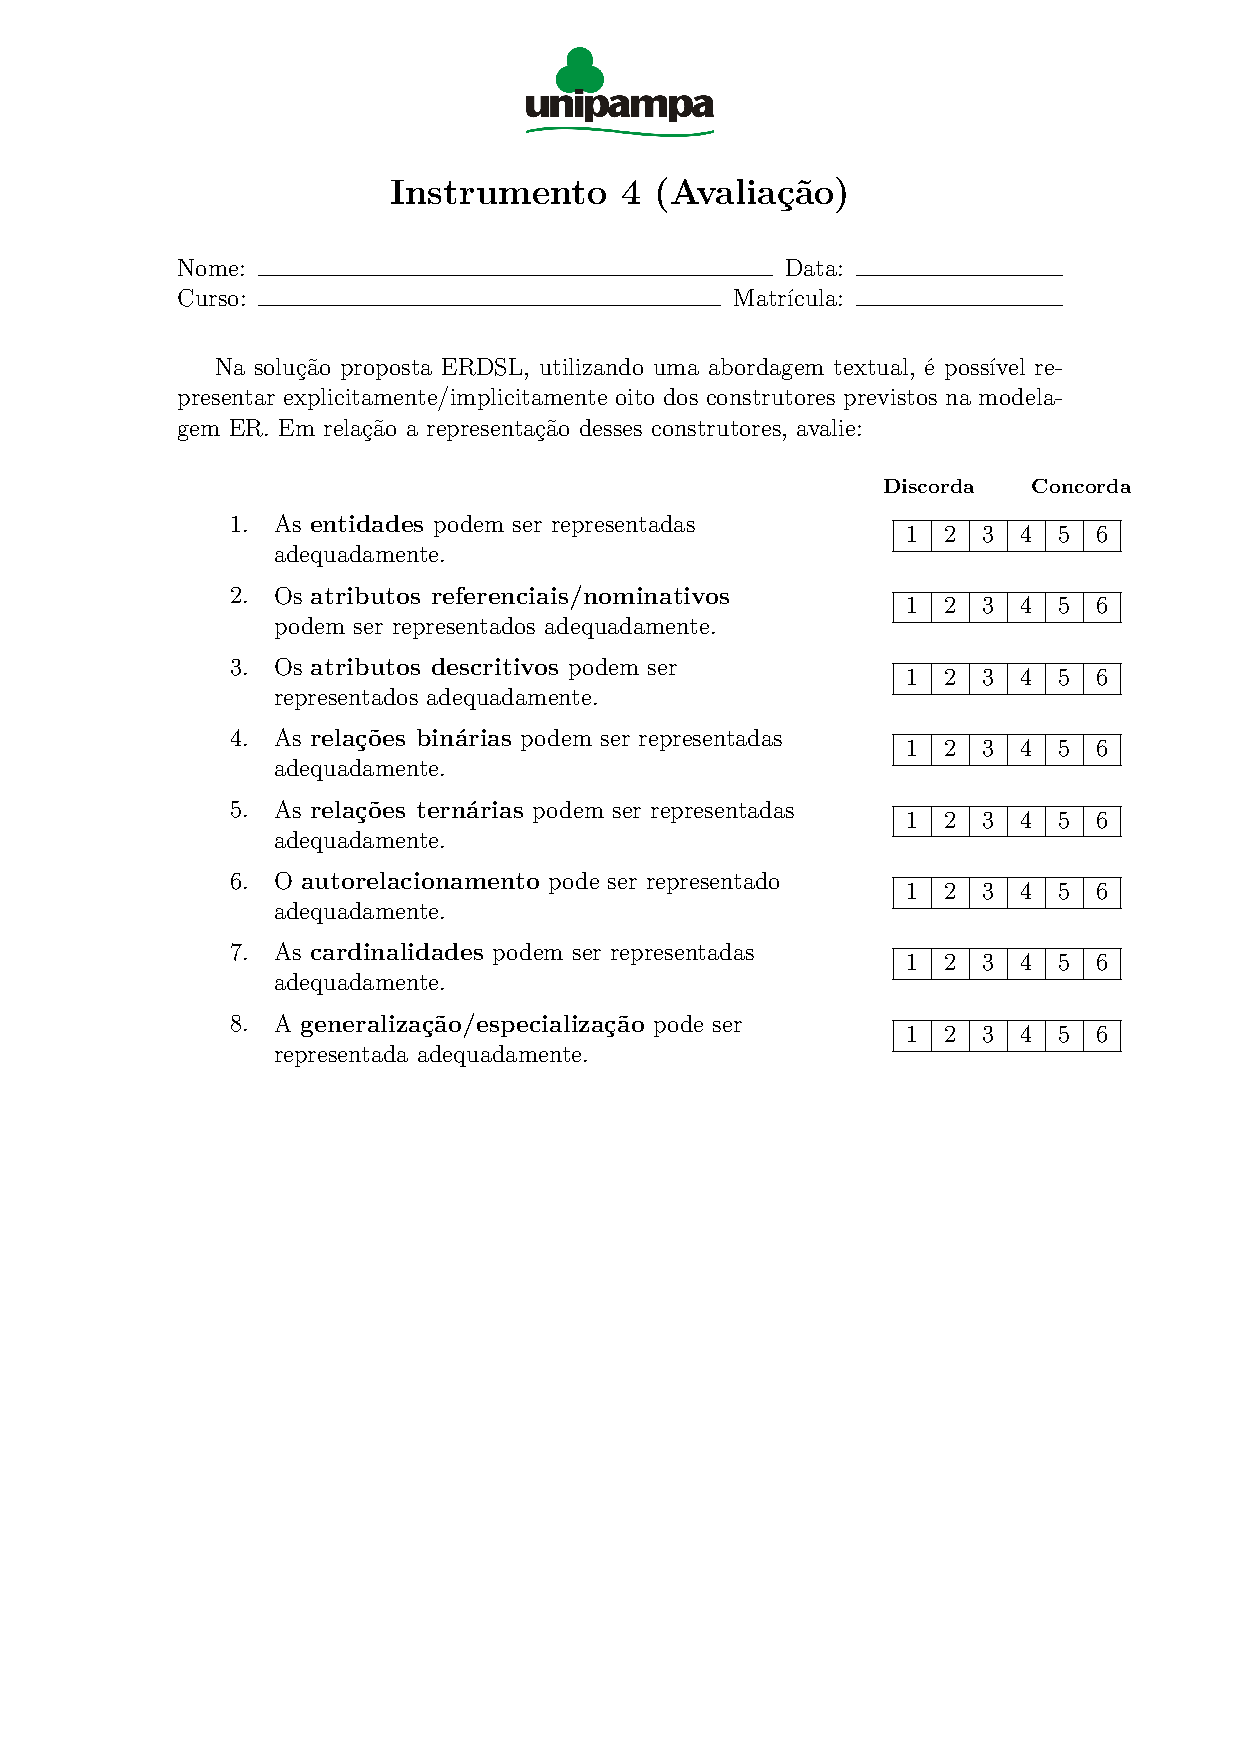
\includepdf[pages=-, frame=true, scale=0.65]{docsApend/expControl/Instrumento4} 
    \end{figure}
\newpage





% %==============================================================================
% \chapter{Primeiro Apêndice}
% %==============================================================================

% De acordo com a ABNT:

% \begin{quotation}
% Apêndice (opcional): texto utilizado quando o autor pretende complementar sua argumentação. São identificados por letras maiúsculas e travessão, seguido do título. Ex.: APÊNDICE A - Avaliação de células totais aos quatro dias de evolução

% Anexo (opcional): texto ou documento \textbf{não elaborado pelo autor} para comprovar ou ilustrar. São identificados por letras maiúsculas e travessão, seguido do título. Ex.: ANEXO A - Representação gráfica de contagem de células
% \end{quotation}

% Tais definições (e outras) podem ser encontradas na NBR 14724-2001 Informação e documentação - trabalhos acadêmicos\footnote{http://www.firb.br/abntmonograf.htm}.


% %==============================================================================
% \chapter{Segundo Apêndice}
% %==============================================================================

% Pode ser que tenha outro...


\end{apendicesenv}
